\begin{figure}
\centering
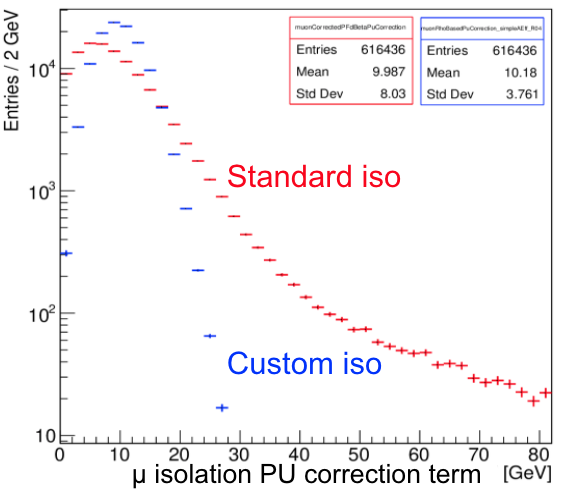
\includegraphics[width=0.44\textwidth]{figures/selection/CustomVsStandardMuIsoPUcorrection_2018emuTTbar_PCR.png}
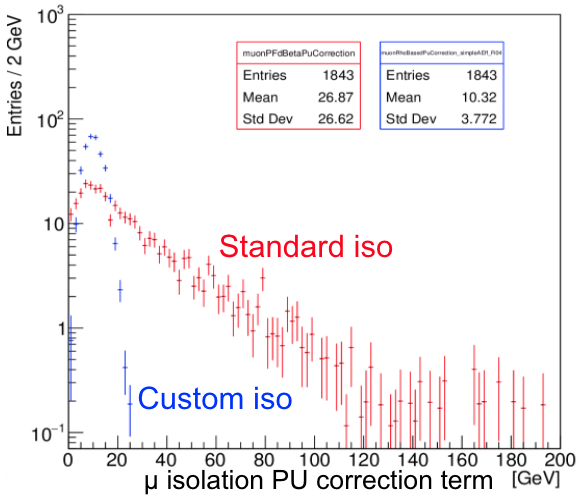
\includegraphics[width=0.45\textwidth]{figures/selection/CustomVsStandardMuIsoPUcorrection_2018emuTTbar_500To1000um.png}
\caption{Comparison of the the muon isolation pileup correction term in the standard muon isolation and the modified muon isolation in simulated \ttbar events that pass the 2018 $\Pe\Pgm$ preselection. Muon \ad is constrained to be less than \SI{100}{\um} in the plot on the left and between \num{500} and \SI{1000}{\um} in the plot on the right.}
\label{iso_pu_term_comparison}
\end{figure}

\begin{figure}\fxnote{weirdly low resolution}
\centering
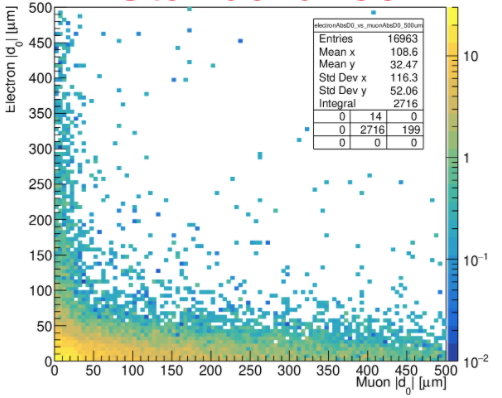
\includegraphics[width=0.45\textwidth]{figures/selection/StandardIso_ElectronD0vsMuonD0_2018emuTTbar.png}
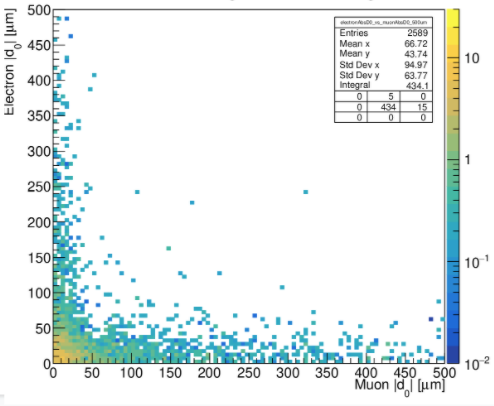
\includegraphics[width=0.44\textwidth]{figures/selection/CustomIso_ElectronD0vsMuonD0_2018emuTTbar.png}
\caption{The distribution of \ttbar simulated events in the plane defined by electron \ad and muon \ad. The standard isolation is applied in the plot on the left, and the modified isolation is applied in the plot on the right, and the events in both plots are required to pass the remaining 2018 $\Pe\Pgm$ preselection criteria and the additional constraint that the parent of at least one lepton is a heavy-flavor meson. }
\label{iso_performance_comparison}
\end{figure}

\begin{figure}\fxnote{weirdly low resolution}
\centering
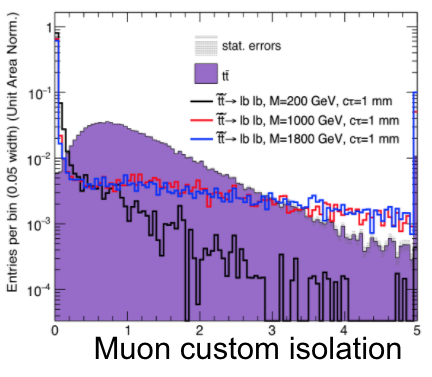
\includegraphics[width=0.5\textwidth]{figures/selection/MuonCustomIso_TTbar_Signal.png}
\caption{The muon modified isolation distribution for simulated \ttbar background and \stoptolb signal events that pass the 2018 $\Pe\Pgm$ preselection with no isolation criterion applied.}
\label{iso_signal_bg}
\end{figure}